\documentclass{beamer}

\usepackage[utf8]{inputenc}
\usetheme{default}

\usepackage{listings}
\lstset{
basicstyle=\small\ttfamily,
columns=flexible,
breaklines=true
}

\usepackage{epstopdf}
\usepackage{multicol}
\usepackage{caption}

\makeatletter
\DeclareMathSizes{\f@size}{10}{7}{7}
\makeatother

\title[66.20/86.37]{U.B.A. - Facultad de Ingeniería\\\vspace{0.25cm} 66.20/86.37 Organización de Computadoras
\\Arquitecturas}
\author{Práctica}
\date{1$^{er}$ cuatrimestre 2020}


\begin{document}
\begin{frame}
\titlepage % Print the title page as the first frame
\end{frame}

\begin{frame}
\frametitle{Clasificación de ISAs}
\begin{center}
 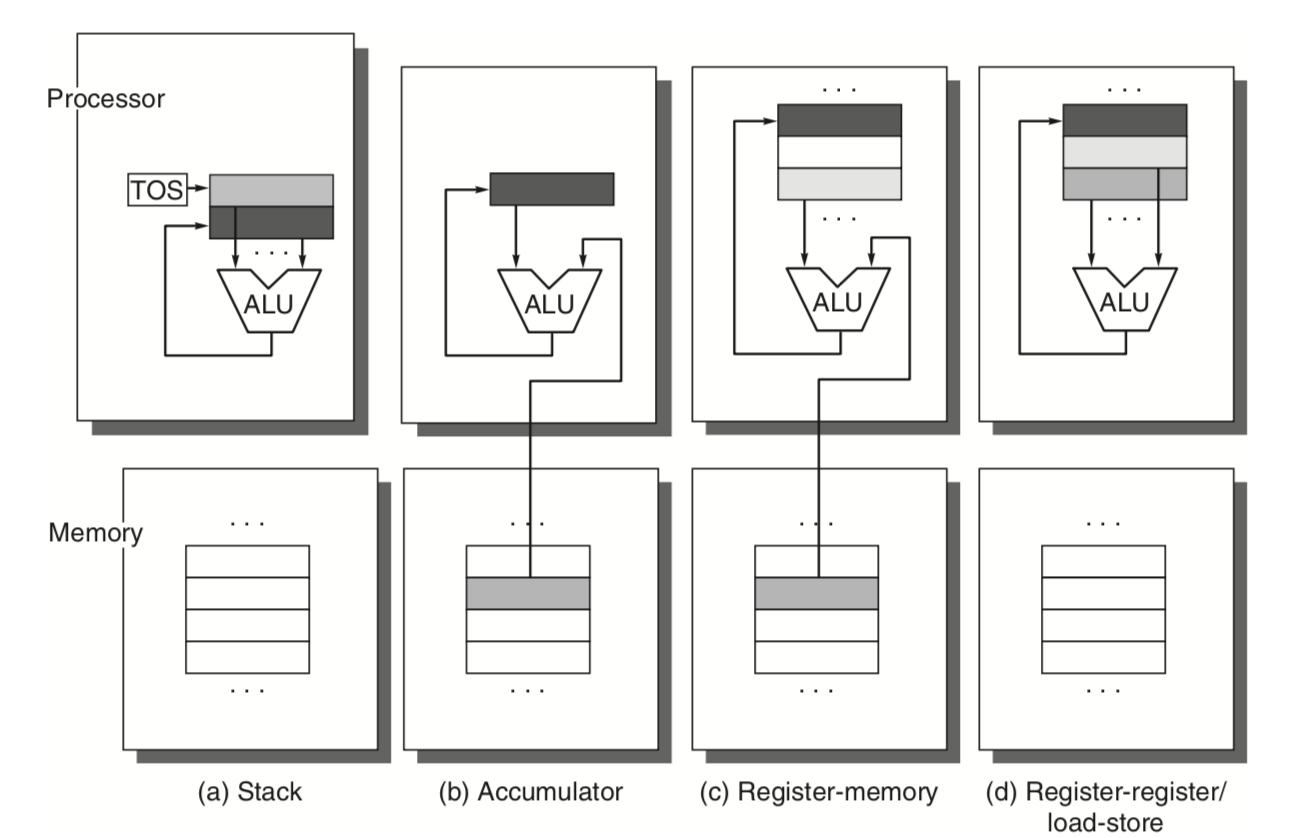
\includegraphics[scale=.45,keepaspectratio=true]{ISA.png}
\end{center}
\end{frame}

\begin{frame}
 \frametitle{Clasificación de ISAs}
 \begin{itemize}
  \item Modelo de pila: 
Los operandos están implícitamente en el tope del stack y el hardware debe evaluar la expresión en un solo orden y cargar un operando múltiples veces.
\item Modelo de acumulador: 
En una arquitectura de acumulador un operando está implícito en el acumulador.
\item Modelo de registros de propósito general: 
Aquí se tienen únicamente operandos explícitos, ya sea que estén ubicados en registros o en memoria.
\item Modelo de carga y almacenamiento: 
En este tipo de arquitectura, la memoria solo puede ser accedida a través de instrucciones de carga y almacenamiento (load/store). 
 \end{itemize}
\end{frame}


\begin{frame}
 \frametitle{Tipo de instrucciones en MIPS}
 \begin{itemize}
  \item Load / Store: únicas que acceden a memoria.
  \item Computational: realizadas en la ALU.
  \item Jump / Branch: saltos incondicionales y condicionales.
  \item Miscelaneas: Serialización de instrucciones, Excepciones (syscall), Moves condicionales, Prefetch, NOPs.
  \item Coprocessors y FPU.
 \end{itemize}
\end{frame}

\begin{frame}
 \frametitle{Ejercicio 2.1 CAAQA 3ed}
 
Asumir que los valores A, B, C, D y E residen en memoria, que el opcode de la instrucción es de 8 bits, las direcciones de memoria son de 64 bits y las direcciones de registro son de 6 bits.

\begin{enumerate}[a.]
 \item Por cada arquitectura del conjunto de instrucciones mostradas en el primer slide ?`Cuántas direcciones o nombres aparecen en cada instrucción para calcular  C = A + B y cuál es el tamaño total del código?

 \item Algunas ISAs de la figura del primer slide destruyen los operando durante el cómputo y trae una consecuencia de performance. Para cada arquitectura escribir la secuencia de código para calcular C = A + B seguido de D = A - E. En el código, indicar cada operando que se destruye durante la ejecución e indicar en cada una el “overhead”  que se incluye como solución. Dar el tamaño en total del código, los datos que son movidos de o hacia memoria y el overhead de cada secuencia de código.
\end{enumerate}
\end{frame}

\begin{frame}
 \frametitle{Ejercicio 2.1 CAAQA 3ed - Resolución}
 \begin{enumerate}[a.]
 \item
\end{enumerate}
\begin{center}
\begin{figure}
 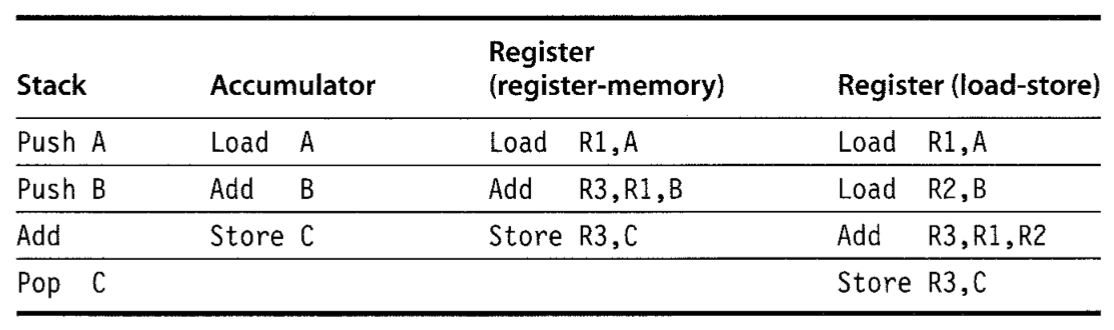
\includegraphics[scale=.45,keepaspectratio=true]{Ejercicio21a.png}
\caption*{C = A + B}
\end{figure}
\end{center}
 \end{frame}

\begin{frame}
 \frametitle{Ejercicio 2.1 CAAQA 3ed - Resolución}
 \begin{enumerate}[b.]
 \item
\end{enumerate}
\begin{center}

\begin{figure}
\caption*{Code size = opcode + memory  operand = 8 bits + 64 bits = 72 bits}
 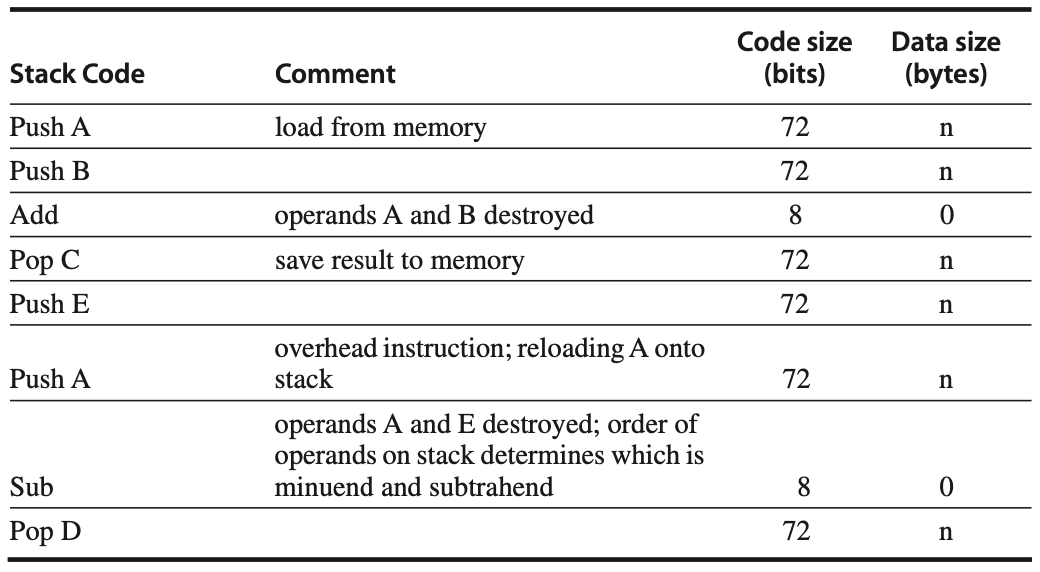
\includegraphics[scale=.45,keepaspectratio=true]{Ejercicio21b1.png}
\caption*{El tamaño del código es 448 bits (56 bytes), el total de datos movidos de ó hacia memoria es  6n bytes. Hay una instrucción y un operando que generan overhead.}
\end{figure}

\end{center}
 \end{frame}

\begin{frame}
 \frametitle{Ejercicio 2.1 CAAQA 3ed - Resolución}
 \begin{enumerate}[b.]
 \item
\end{enumerate}
\begin{center}
\begin{figure}
 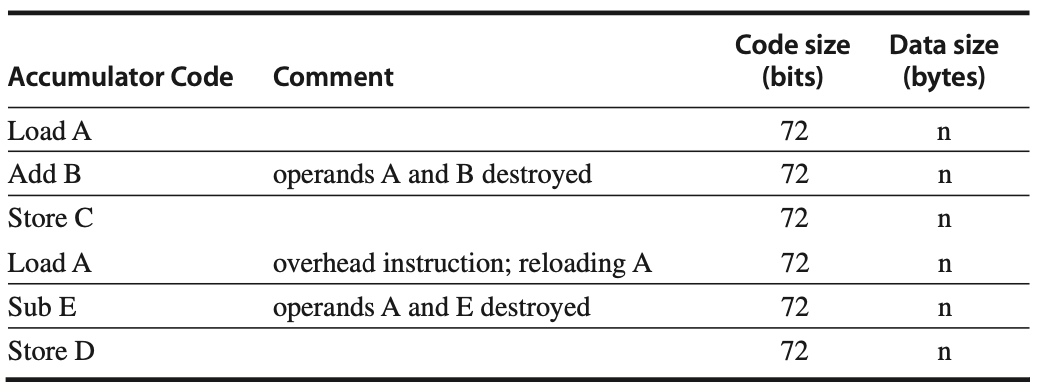
\includegraphics[scale=.45,keepaspectratio=true]{Ejercicio21b2.png}
\caption*{El tamaño del código es 432 bits (54 bytes), el total de datos movidos de ó hacia memoria es 6n bytes. Hay una instrucción y un operando que generan overhead.}
\end{figure}
\end{center}
 \end{frame}
 
 \begin{frame}
 \frametitle{Ejercicio 2.1 CAAQA 3ed - Resolución}
 \begin{enumerate}[b.]
 \item
\end{enumerate}
\begin{center}
\begin{figure}
\caption*{Code size = opcode + register operand + memory  operand = 8 bits + 6 bits + 64 bits = 78 bits}
 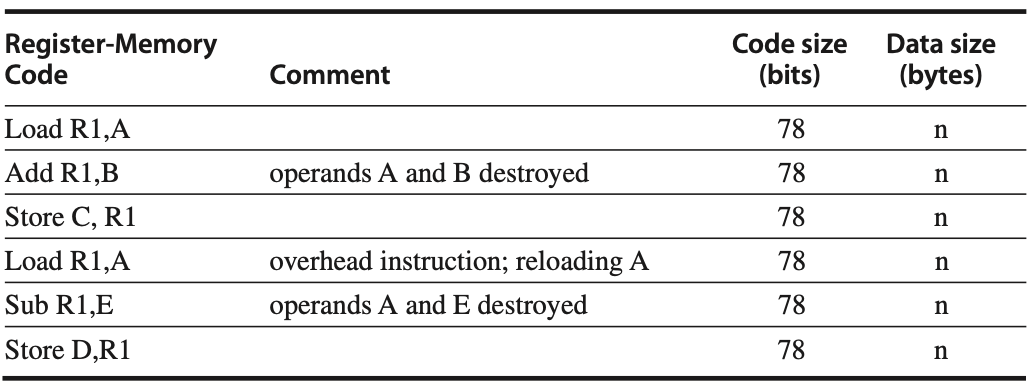
\includegraphics[scale=.45,keepaspectratio=true]{Ejercicio21b3.png}
 \caption*{El tamaño del código es 468 bits (59 bytes), el total de datos movidos de ó hacia memoria es 6n bytes. Hay una instrucción y un operando que generan overhead.}
\end{figure}
\end{center}
 \end{frame}

 
 \begin{frame}
 \frametitle{Ejercicio 2.1 CAAQA 3ed - Resolución}
 \begin{enumerate}[b.]
 \item
\end{enumerate}
\begin{center}
\begin{figure}
 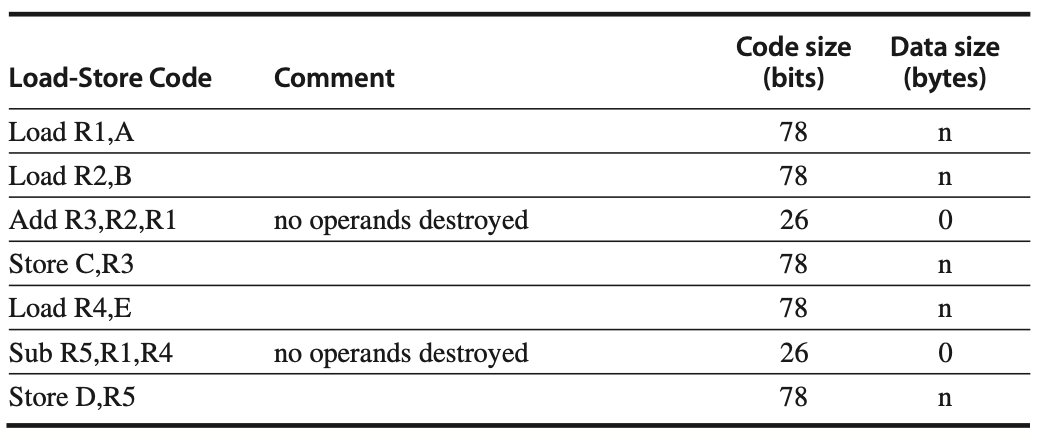
\includegraphics[scale=.45,keepaspectratio=true]{Ejercicio21b4.png}
 \caption*{El tamaño del código es  442 bits (55 bytes), el total de datos movidos de ó hacia memoria es 5n bytes. No hay overhead en las instrucciones ni en los operando de datos.}
\end{figure}
\end{center}
 \end{frame}


\begin{frame}
 \frametitle{Ejercicio 2.2 CAAQA 3ed}
Algunas operaciones con dos operando no son conmutativas (la resta por ejemplo). ?`Qué ventajas y desventajas en las arquitecturas de pila, acumulador y carga-almacentamiento existen cuando se ejecuta operaciones no conmutativas?
\end{frame}

\begin{frame}
 \frametitle{Ejercicio 2.2 CAAQA 3ed - Resolución}
\begin{itemize}
 \item \textbf{Stack}
  \begin{itemize}
    \item Ventajas: El tamaño de las instrucciones es pequeño porque no hay que ubicar los operando o el resultado.
    \item Desventajas: En general los operando tienen que estar en el orden correcto. Una instrucción útil podría ser para intercambiar el tope de pila.
  \end{itemize}

\item \textbf{Acumulador}
\begin{itemize}
\item Ventajas: La codificación de las instrucciones es pequeña ya que hay un solo operando.
\item Desventajas: Lo mismo que para la pila, los operando deben estar en el orden correcto. Una instrucción útil podría ser para intercambiar el contenido del acumulador con cualquier ubicación de un operando.
\end{itemize}

\item \textbf{Load-Store}
\begin{itemize}
\item Ventajas: Ya que los operando están en registros se pueden intercambiar cuando sea necesario.
\item Desventajas: Tamaño más grande para encodear las instrucciones.
\end{itemize}
\end{itemize}

\end{frame}


\begin{frame}
 \frametitle{Endianess}
Todo el conjunto de instrucciones es direccionado por bytes y se provee acceso por bytes (8 bits), mitad de palabra (half words) (16 bits), por palabra (words) (32 bits).

\bigskip

Hay dos convenciones para ordenar los bytes en un objeto. \textbf{Little Endian} y \textbf{Big Endian}.
 \end{frame}
 
\begin{frame}
 \frametitle{Endianess}

El orden \textbf{Little Endian} coloca el byte cuya dirección "x . . . x000” en la posición menos significativa. Los bytes entonces son numerados:

  \begin{center}
 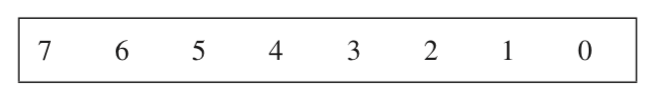
\includegraphics[scale=.7,keepaspectratio=true]{little_endian.png}
\end{center}


El orden \textbf{Big Endian} coloca el byte cuya dirección es “x . . . x000”  en la posición más significativa. Los bytes entonces son numerados:

\begin{center}
 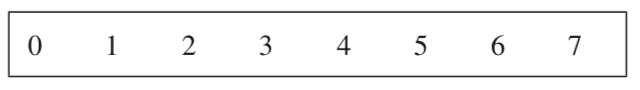
\includegraphics[scale=.7,keepaspectratio=true]{big_endian.png}
\end{center}

 \end{frame}


\begin{frame}
 \frametitle{Alineación}
 En varias computadoras, los accesos a objetos más grandes que un byte deben estar alineados.
 \begin{itemize}
  \item Un objeto de tamaño s bytes en la dirección de bytes A está alineado si
    A mod s = 0.
  \item Esto se fuerza en muchas arquitecturas porque el hardware accede a
    memoria típicamente alineado a múltiplos de word o double-word.
 \end{itemize}
\bigskip
 ¿Qué puede ocurrir a nivel de accesos a memoria si se accede a datos no alineados y la arquitectura lo permite?
    
\end{frame}

\begin{frame}
 \frametitle{Modos de direccionamiento}
Se presentan varios modos de direccionamiento: 
\begin{multicols}{2}
\begin{itemize}
 \item Register
 \item Immediate
 \item Displacement
 \item Register indirect
 \item Indexed
 \item Direct or Absolute
 \item Memory indirect
 \item Autoincrement
 \item Autodecrement
 \item Scaled
 \end{itemize}
\end{multicols}

MIPS implementa 2 modos de direccionamiento: Immediate y Displacement, ambos con immediate de 16 bits.
    
Usando el registro 0 se consigue Absolute, y con displacement 0 se consigue Register indirect.
\end{frame}

\begin{frame}[fragile]
\frametitle{Modos de direccionamiento}

\begin{lstlisting}
    Immediate:		add	$t1, $t2, 10	
    Displacement:	lw	$t1, 30($t2)
    Absolute:		sb	$t1, 40($0)
    Indirect:		sw	$t1, 0($t2)
\end{lstlisting}
\end{frame}

\begin{frame}
 \frametitle{Ejercicio 2.3 CAAQA 3ed}
 El valor representado por el número hexadecimal 434F 4D50 5554 4552 se almacena en una palabra doble alineada en 64 bits.

 \begin{enumerate}[a.]
  \item Utilizando el arreglo físico de la primera fila en la Figura 2.5, escribir el valor a ser almacenado utilizando el orden de byte Big Endian. Luego, interpretar cada byte como caracter ASCII y debajo de cada byte escribir el caracter correspondiente formando la cadena de caracteres que se almacenaría en el orden Big Endian.
  
  \item Realizar el punto (a.) pero siguiendo el orden Little Endian.

 \end{enumerate}

\end{frame}

\begin{frame}
 \frametitle{Ejercicio 2.3 CAAQA 3ed}
 \begin{center}
 \begin{figure}
 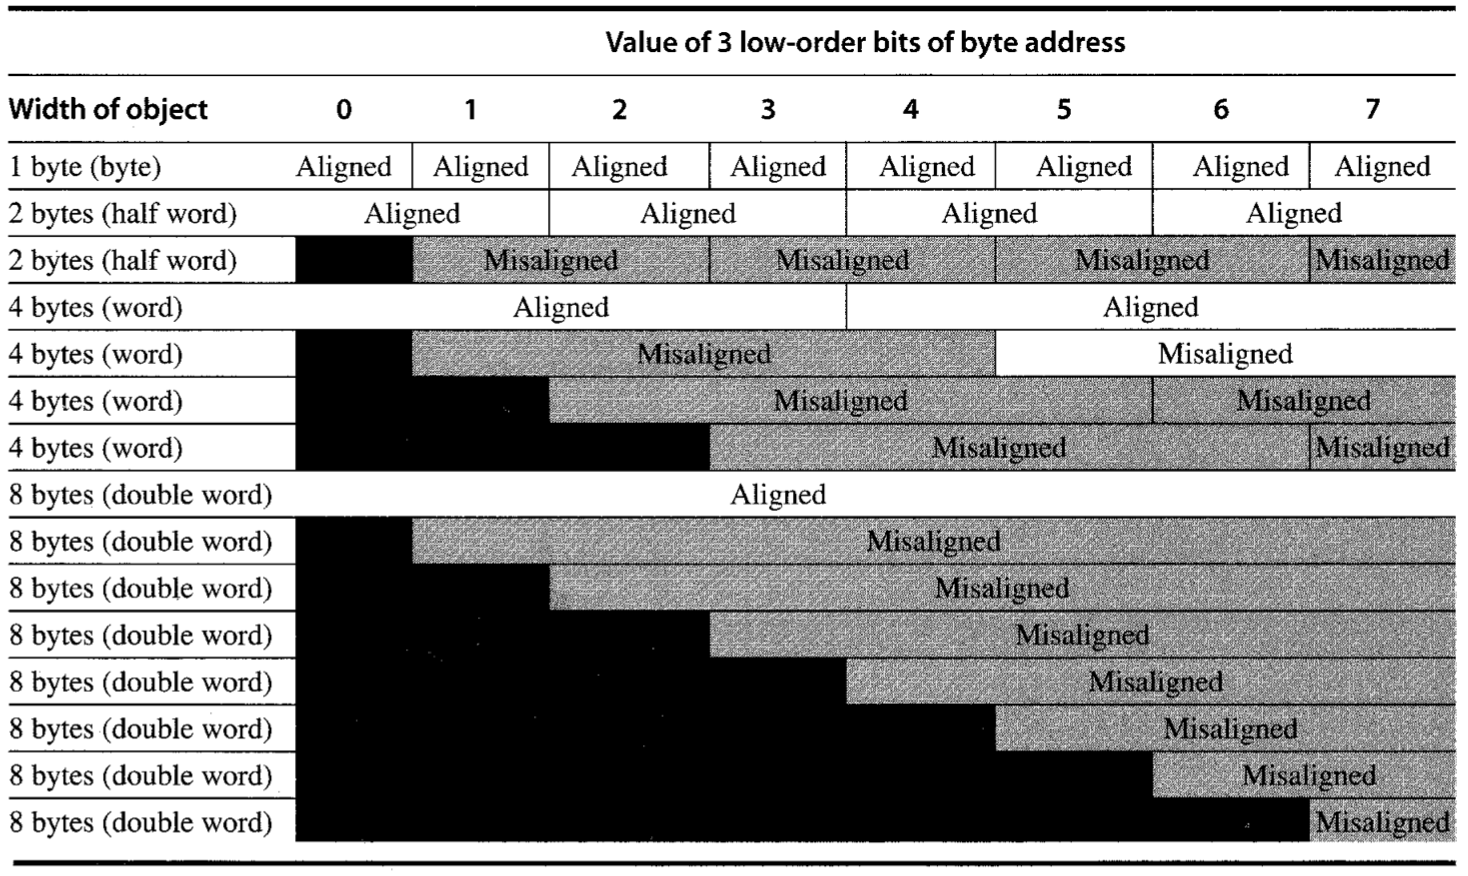
\includegraphics[scale=.35,keepaspectratio=true]{align.png}
 \caption*{Fiigura 2.5: Direcciones de byte alineadas y no alineadas} %Fix this

 \end{figure}

\end{center}
 \end{frame}
 
\begin{frame}
 \frametitle{Ejercicio 2.3 CAAQA 3ed - Resolución}
 
 \fbox{\fbox{43}4F 4D 50 55 54 45 \fbox{52}}  almacenada en una palabra doble alineada en 64 bits.

 \begin{enumerate}[a.]
  \item Big Endian
   \end{enumerate}

\begin{center}
  \begin{tabular}{| c | c | c | c | c | c | c | c | }
    \hline
    43 & 4F & 4D & 50 &55 & 54 & 45 & 52 \\ \hline
    C & O & M & P & U & T & E & R \\ \hline
  \end{tabular}
\end{center}

 \begin{enumerate}[b.]
  \item Little Endian
   \end{enumerate}
  
  \begin{center}
  \begin{tabular}{| c | c | c | c | c | c | c | c | }
    \hline
    52 & 45 & 54 & 55 & 50 & 4D & 4F & 43 \\ \hline
     R & E & T & U & P & M & O & C \\ \hline
  \end{tabular}
\end{center}
   
 \end{frame}

\begin{frame}
 \frametitle{Encoding MIPS} 
 Hay 3 formatos de encoding posibles en MIPS
 \begin{itemize}
  \item I-type (Immediate)
  \item R-type (Register)
  \item J-type (Jump)
 \end{itemize}
\end{frame}

\begin{frame}
 \frametitle{Encoding MIPS} 
 
 \begin{center}
 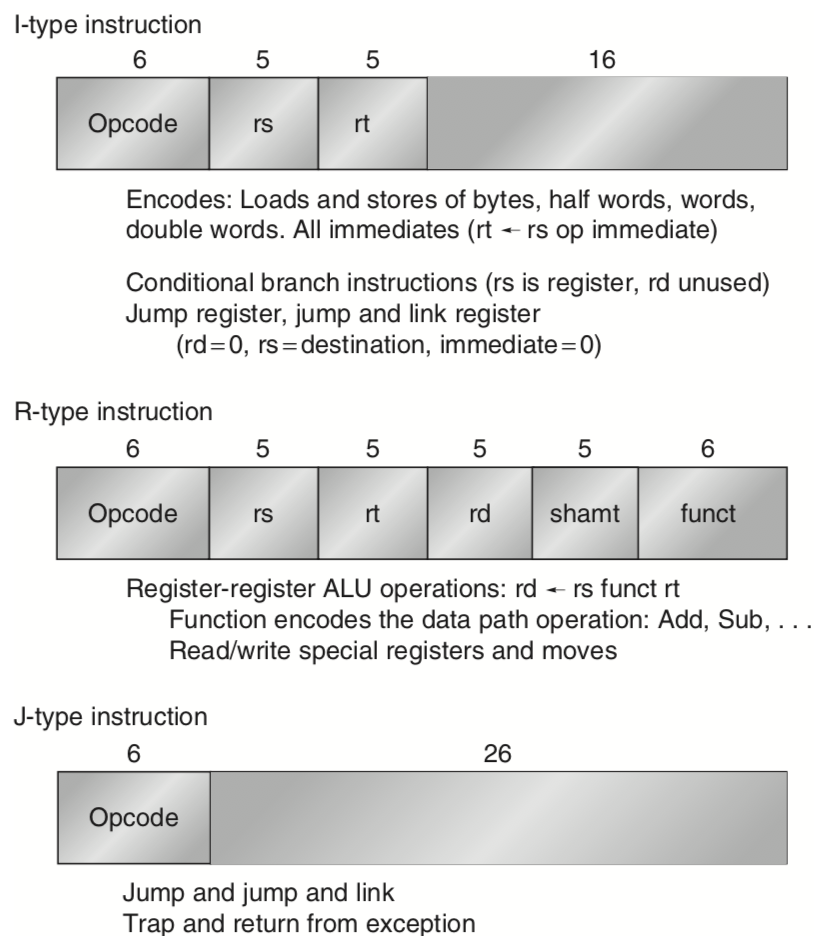
\includegraphics[scale=.4,keepaspectratio=true]{tipos_instruccion.png}
\end{center}
 \end{frame}


\begin{frame}
 \frametitle{Encoding MIPS} 

 Viendo el detalle de las instrucciones J-type vemos que hay un offset de 26 bits left-shifted 2 bits, para formar los 28 lsb de la direccion destino del salto (las regiones de salto están alineadas a 256MB, y la región está determinada por los 4 msb de PC).
 
 \bigskip

 ¿Por qué se puede (y conviene) tomar los 26 bits como desplazados a la izquierda 2 bits?
\end{frame}

\begin{frame}

         \begin{center}
         \begin{table}
         \begin{tabular}{||l|c||}
         \hline
         Instrucción & Frecuencia \\\hline
         \textit{Load} & $26\%$ \\\hline
         \textit{Store} & $10\%$ \\\hline
         Aritméticas & $14\%$ \\\hline
         Comparaciones & $13\%$ \\\hline
         Saltos condicionales & $16\%$ \\\hline
         Saltos incondicionales & $1\%$ \\\hline
         \textit{Call / Return} & $2\%$ \\\hline
         Shift & $4\%$ \\\hline
         Logicas & $4\%$ \\\hline
         Misc. & $5\%$ \\\hline

         \end{tabular}
                           \caption*{\textit{Tabla 1: Mix. de instrucciones}} \label{tab:tabla1} %Fix this
\end{table}
         \end{center}

\end{frame}
     
\begin{frame}[fragile]
 \frametitle{Ejercicio 2.6 CAAQA 3ed}
Varios investigadores han sugerido que incorporar un modo de direccionamiento registro-memoria a una máquina \textit{Load/Store} puede ser conveniente. La idea es reemplazar la siguiente secuencia
 
\begin{lstlisting}
 LOAD   R1, 0(Rb)
 ADD    R2, R2, R1
\end{lstlisting}

por

\begin{lstlisting}
 ADD    R2, 0(Rb)
\end{lstlisting}


Asumir que la nueva instrucción provoca un incremento en el ciclo de clock del $5\%$. Utilizar la frecuencia de instrucciones de la Tabla 1. La nueva instrucción afecta únicamente al ciclo de clock y \underline{no al CPI}.

\end{frame}

\begin{frame}
 \frametitle{Ejercicio 2.6 CAAQA 3ed}
\begin{enumerate}[a.]
\item ¿Qué porcentaje de loads deben ser eliminados en la máquina con la nueva instrucción para tener al menos el mismo rendimiento?
\item Mostrar una secuencia de instrucciones donde un load de R1 seguido inmediatamente por el uso de R1 (con algún tipo de opcode) no podría ser reemplazado por una única instrucción como la propuesta, asumir que el mismo opcode existe.  
\end{enumerate}
\end{frame}

\begin{frame}
 \frametitle{Ejercicio 2.6 CAAQA 3ed - Resolución}
\begin{enumerate}[a.]
\item
\end{enumerate}
Vamos a partir de la ecuación de desempeño antes vista y calcularemos primero reduciendo las instrucciones en su total y no solo los loads. 
\[ CPU Time = CPI \times CC \times IC \]
\begin{eqnarray*}
\text{CPU Time}_{old} &=& CPI_{old} \times CC_{old} \times IC_{old} \\
\text{CPU Time}_{new} &=& CPI_{new} \times CC_{new} \times IC_{new} \\
&=& CPI_{old} \times (CC_{old} \times 1.05) \times (IC_{old} - R) \\
\end{eqnarray*}
Despejando R, tenemos que cantidad de $IC_{old}$ habría que reducir
\[R = 0.048 \times IC_{old} \]

%Entonces tenemos que reducir el $4.8 \% / 26 \% = 18.4\% $ de loads
Entonces tenemos que reemplazar el $\frac{0.048 \times IC_{old}}{IC_{old} \times 0.26 \text{loads} }= 18.4\% $ loads por la nueva instrucción.

\end{frame}

\begin{frame}[fragile]
 \frametitle{Ejercicio 2.6 CAAQA 3ed - Resolución}
\begin{enumerate}[b.]
\item
\end{enumerate}
Consideremos la secuencia
\begin{lstlisting}
LOAD 	R1, 0(R1)
ADD	R1, R1, R1
\end{lstlisting}
El resultado que se escribe en R1 es $MEM[0 + R1] + MEM[0 + R1]$
En el caso de reemplazar esa secuencia por la instrucción
\begin{lstlisting}
ADD	R1, 0(R1)
\end{lstlisting}

El resultado en R1 es $R1 + MEM[0 + R1]$, que si en R1 tenemos  $MEM[0 + R1]$ daría lo mismo pero es algo que no se puede garantizar.
\end{frame}

\begin{frame}
 \frametitle{Ejercicio 2.11 CAAQA 3ed}
            Calcular el \underline{CPI Efectivo} para MIPS utilizando la Tabla 1. Asumir que se obtuvieron los siguientes CPI para instrucciones.

            \begin{center}
            \begin{tabular}{||l|c||}
            \hline
            Instrucción & Ciclos \\
            \hline
            ALU & $1,0$ \\\hline
            \textit{Load}/\textit{Store} & $1,4$ \\\hline
            Saltos condicionales & \\\hline
            \multicolumn{1}{||r|}{Tomados} & $2,0$ \\\hline
            \multicolumn{1}{||r|}{No Tomados} & $1,5$ \\\hline
            Saltos & $1,2$ \\\hline
            \end{tabular}
            \end{center}

            Asumir que el $60\%$ de los saltos son tomados.
 
\end{frame}

\begin{frame}
 \frametitle{Ejercicio 2.11 CAAQA 3ed - Resolución}
 Vamos a llevar el mix de instrucciones de la Tabla 1 a estas cuatro categorías para calcular el CPI. Tenemos que el 53\% de las instrucciones son ALU (tardan 1 ciclo en promedio), las instrucciones L/S son el 36 \% y tardan 1.4 ciclos, saltos condicionales 16\% (depende si se toman o no) y saltos son el 1 \% y tardan 1.2 ciclos. Con lo cual podemos calcular el CPI efectivo
 
 \[ \overline{CPI} = \frac{\sum_i IC_i \times CPI_i}{IC}\]
 
 \[ \overline{CPI} = 0.53 \times 1 + 0.36 \times 1.4 + 0.01 \times 1.2 + \underbrace{0.16 \times ( \underbrace{0.6 \times 2}_{tomados} + (1-0.6) \times 1.5)}_{saltos} \]

\end{frame}
\begin{frame}[fragile]
 \frametitle{Ejercicio 2.12 CAAQA 3ed}
 
 Considerar el agregado de un nuevo modo de acceso a MIPS. El nuevo modo suma dos registros y un valor de offset de 11 bits con signo para obtener la dirección efectiva. Utilizar el porcentaje de instrucciones indicado en la Tabla 1. El compilador pasa de las instrucciones: 
    
\begin{lstlisting}
ADD     R1, R1, R2
LW      Rd, 100(R1)	(or Store)
 \end{lstlisting}

A utilizar:
\begin{lstlisting}
LW    Rd, 100(R1,R2)
 \end{lstlisting}

\end{frame}

\begin{frame}[fragile]
 \frametitle{Ejercicio 2.12 CAAQA 3ed}
\begin{enumerate}[a.]
 \item Asumir que el nuevo modo de acceso es usado por el $10\%$ de los \textit{loads} y \textit{stores}. ¿Cuál es el porcentaje de IC nuevo comparado con la tasa original?
\item Si el nuevo modo de direccionamiento aumenta en 5\% el tiempo de clock, ¿Cuál computadora será más rápida y por cuanto?
\item Describa una situación que limite el porcentaje de reemplazos realizado.

\end{enumerate}

\end{frame}
\end{document}
